
%\begin{savequote}[6cm]
%<< truc
%\qauthor{Test}
%\end{savequote}

\chapter{Caractérisation des architectures NUMA}\label{chap:contrib:characterization}
\chaptertoc

\section{Exécution précise de noyaux}\label{sec:contribs:outil}

\subsection{Besoins pour un outil spécifique}

Les résultats de la section précédente montrent que l'on peut tout à fait étudier le comportement global d'une application sur une machine. On peut évidemment observer aussi les variations de ce comportement global lorsqu'on change certains détails, via l'utilisation par exemple de \emph{numactl}.

En revanche, si l'on connait bien son application, on a envie de pouvoir étudier le comportement précis de certaines parties critiques de l'application afin de pouvoir identifier ce qui cause le comportement global.

La suite naturelle de cette identification est de déterminer s'il y a des améliorations possibles pour ce comportement local, et comment l'améliorer en pratique.

Dans le cas d'une application à base de flots de données, chaque partie de l'application est bien identifiée, et correspond à un noeud dans le graphe de tâches.
Toutes les données manipulées par une partie de l'application sont facilement identifiées également, puisqu'il s'agit des connexions entre les noeuds du graphe de tâches.

Dans le contexte d'une machine NUMA, le temps d'exécution d'une tâche dépend à la fois du placement de son exécution, ainsi que du placement de ces données. On a donc envie de pouvoir modéliser le comportement individuel de chaque type de tâche en fonction de son placement et du placement des données.

Une fois cela fait, cela permettra d'identifier des potentielles variations de comportement, et ajuster les heuristiques d'ordonnancement pour prendre en compte ces variations.

C'est à ce besoin que répond NOMDEL4OUTIL : permettre à l'utilisateur de définir ce qu'il exécute et où, et garantir cette exécution, avec un certain nombre de variables observables.

Dans la suite de ce chapitre, on appellera l'ensemble des paramètres décrivant cette expérience un \emph{scenario}.

\subsection{Description d'un scenario}

Ce qu'on appelle ici un \emph{scenario} n'est ni plus ni moins que la description d'une expérience.
Par exemple on pourrait vouloir "observer les performances en gigaflops d'une multiplication de matrices carrées sur le coeur 0 d'une machine".
C'est un scenario simple, et l'exemple que l'on prendra pour illustrer les points un peu plus formel qui vont suivre.

En pratique un scenario est défini de la manière suivante :
\begin{itemize}
 \item Un ensemble de données et variables
 \item Une liste d'actions à effectuer
 \item Un ensemble de caractéristiques à observer
\end{itemize}

Cette définition très générique permet beaucoup de flexibilité, et les sections suivantes précisent les différentes caractéristiques de ces points, ainsi que des exemples concrêt d'utilisation.

Il est important que le format de description d'un scenario soit humainement lisible, et ne conduise pas à une recompilation systématique du programme. C'est donc une description en YAML qui a été choisie.

\subsubsection{Données et variables}

Elles sont indispensables car c'est la dessus que vont se baser les actions du scenario.

L'utilisateur doit fournir les noms et type des variables utilisées en paramètres des différents noyaux, elles peuvent être réutilisées par différents noyaux, mais dans tous les cas l'utilisateur est le seul responsable de leur gestion.

En pratique ces variables peuvent soit être des constantes, ou bien être initialisées par une action dans le scénario.

Pour revenir à l'exemple du scenario simple ou l'on souhaite exécuter une multiplication de matrices carrées - |dgemm| - sur un coeur donné, nous avons besoin de trois matrices |a|, |b|, et |c|, ainsi que d'une taille de bloc, |block_size|.

Voici concrêtement à quoi ressemblerait la déclaration de ces données :

\begin{lstlisting}[language=yaml,caption=Exemple de déclaration de variables,label=lst:tool:data-example]
data:
  - a:
    - type: "double *"
  - b:
    - type: "double *"
  - c:
    - type: "double *"
  - block_size:
    - type: "int"
    - value: 256
\end{lstlisting}

\subsubsection{Actions}

C'est là où on décrit effectivement les noyaux exécutés au cours du scénario.
L'utilisateur indique une série d'actions à exécuter, et avec quels paramètres.

Chaque action peut avoir les caractéristiques suivantes :
\begin{itemize}
  \item core: nombre entier indiquant le coeur sur lequel exécuter l'action.
  \item kernel: chaine de caractères avec le nom de l'action, correspondant à un noyau connu du programme.
  \item params: liste de variables à passer à l'action, leur nom doit correspondre à des données déclarées dans la section précédente.
  \item repeat: nombre entier indiquant le nombre de fois que cette action doit être répétée.
  \item sync: booléen indiquant s'il faut synchroniser le démarrage de cette action avec celui des autres actions présentes dans les file d'attente des autres coeurs.
\end{itemize}

Si on continue dans l'exemple simple d'une multiplication de matrices carrées, il faut que l'on définisse les actions suivantes : l'initialisation de chaque matrice, le lancement du dgemm une fois que ces matrices sont initialisées.
Afin d'avoir une mesure plus précise du comportement du noyau, on peut indiquer une répétition du noyau, ici on choisi 50 pour l'exemple.

Voici en pratique à quoi ressemblerait un tel scenario :
\begin{lstlisting}[language=yaml,caption=Exemple de déclaration d'actions,label=lst:tool:actions-example]
actions:
  - kernel: init_blas_bloc
    sync: false
    params: 
    - a
    - block_size
    core: 0
    # Pour l'initialisation, un seul appel suffit
    repeat: 1
  - kernel: init_blas_bloc
    sync: false
    params: 
    - b
    - block_size
    core: 0
    repeat: 1
  - kernel: init_blas_bloc
    sync: false
    params: 
    - c
    - block_size
    core: 0
    repeat: 1
  - kernel: dgemm
    # Les actions sont executees dans l'ordre de declaration, pour un seul dgemm c'est inutile de synchroniser
    sync: false
    params: 
    - a
    - b
    - c
    - block_size
    core: 0
    # Ici c'est le noyau de calcul, on veut donc le repeter
    repeat: 50
\end{lstlisting}

Simplement exécuter ces actions ne nous donnera pas grand chose, il faut donc définir un ensemble de paramètres à observer.

\subsubsection{Observateurs}

L'outil propose un certain nombre de caractéristiques observables :

\begin{itemize}
  \item le temps passé dans l'action (en millisecondes).
  \item pour les noyaux d'algèbre linéaire, la performance de l'action en Gflops.
  \item des compteurs de performances à travers PAPI
\end{itemize}

En continuant sur notre exemple, voici à quoi ressemblerait la section du scénario si nous souhaitions observer la performance de la multiplication de matrice en Gflops, le nombre de cycles passé dans l'action, ainsi que le nombre de cache miss au niveau 3 généré par l'action.

\begin{lstlisting}[language=yaml,caption=Exemple de déclaration d'observateurs,label=lst:tool:watchers-example]
watchers:
  flops_dgemm:
    # Le nombre de flops depend de la taille de bloc,
    # il faut donc la donner en parametre
    - block_size
  papi:
    - PAPI_TOT_CYC
    - PAPI_L3_TCM
\end{lstlisting}

\subsection{Design de l'outil}

Afin de garantir un minimum de "bruit" lors des expériences, il fallait que l'archicture de l'outil soit simple, avec peu de logique relative au contrôle de l'exécution des tâches.

Le flot d'exécution est le suivant :

\paragraph{Lecture et analyse du scenario}
L'outil charge le scenario fourni par l'utilisateur, créer les différentes données, et analyse les actions pour déterminer l'ensemble des coeurs physiques qui seront utilisés au cours des actions.

\paragraph{Déroulement des actions}
Pour chacun des coeurs utilisés, un thread est créé et attaché à ce coeur. De plus, une queue d'actions (FIFO) est créée pour ce thread.
L'ensemble des actions sont poussées dans les tâches correspondantes dans l'ordre du fichier.

Dès que les threads sont créés ils commencent à exécuter les actions prêtes ; avant et après chaque actions l'ensemble des observateurs pour cette actions sont appelés afin de les collecter pour cette action.

Lorsque la dernière action du scenario est terminée, l'ensemble des données des observateurs est affiché à l'utilisateur sur la sortie standard.

\subsection{Exemples de noyaux}

\subsubsection{Test de bande passante}

Noyau naïf pour estimer la bande passante noeud à noeud

\subsubsection{dgemm naif}

cf les perf plus haut, pour vérifier que le comportement des caches miss était pas lié à l'implem.


\subsection{Application aux noyaux de Cholesky}

On a identifié les noyaux BLAS important dans la section~\ref{chap:contribs:apps:kastors:cholesky}.

\subsubsection{Quelles caractéristiques observer ?}
Perf ctr, perfs tout court

\paragraph{Impact de la taille de bloc}

TODO : ajouter des courbes
Meilleur cas : tout local, quelques tailles < L2, < L3, > L3

\paragraph{Impact des accès distants}

TODO : ajouter des courbes
Pire cas : tout distant, quelques tailles < L2, < L3, > L3

\subsubsection{Impact de la bibliothèque BLAS}

OpenBLAS, MKL, ATLAS
matter for top perf, not for overall behavior

\subsection{Conclusion : modélisation de base possible}


\section{Présentation et caractéristiques des machines}\label{sec:contribs:machines}

Nous présentons dans cette sections deux machines NUMA de générations différentes et au caractéristiques assez différentes.
La première, \emph{idchire}, est basée sur des processeurs Intel Sandy Bridge, et possède un nombre important de nœuds NUMA.
La seconde, \emph{brunch}, est basé sur des processeurs Intel plus récents de la génération Broadwell, et dispose d'un nombre assez faible de nœud NUMA.

\subsection{idchire}\label{sec:contribs:machines:idchire}


Cette machine est équipée de 24 processeurs Intel(R) Xeon(R) CPU E5-4640 (Sandy Bridge), cadencés à 2.4 GHz.
Chacun de ce processeurs est associé à 31 Go de RAM pour former un nœud NUMA, ils disposent de 8 cœurs physiques partageant 20 Mo de cache L3 (20-ways associatif).
Chacun des cœur à accès à 32 Ko de cache L1 (données) et 256 Ko de cache L2 (8-ways associatif).
Les latences et bandes passantes relatives à chacun des niveaux de cache sont présentées dans le tableau~\ref{tab:synthese-processeurs}.

La machine entière dispose donc de 192 cœurs physiques, et de 744 Go de RAM.
Les processeurs Sandy Bridge disposent de l'extension vectorielle AVX, permettant d'effectuer 4 additions et 4 multiplication de nombres flottant à double précision en un cycle, portant le pic de performance théorique de la machine à 3.6 TFLOPs.

\subsubsection{Topologie}

\begin{figure}[ht]
  \centering
  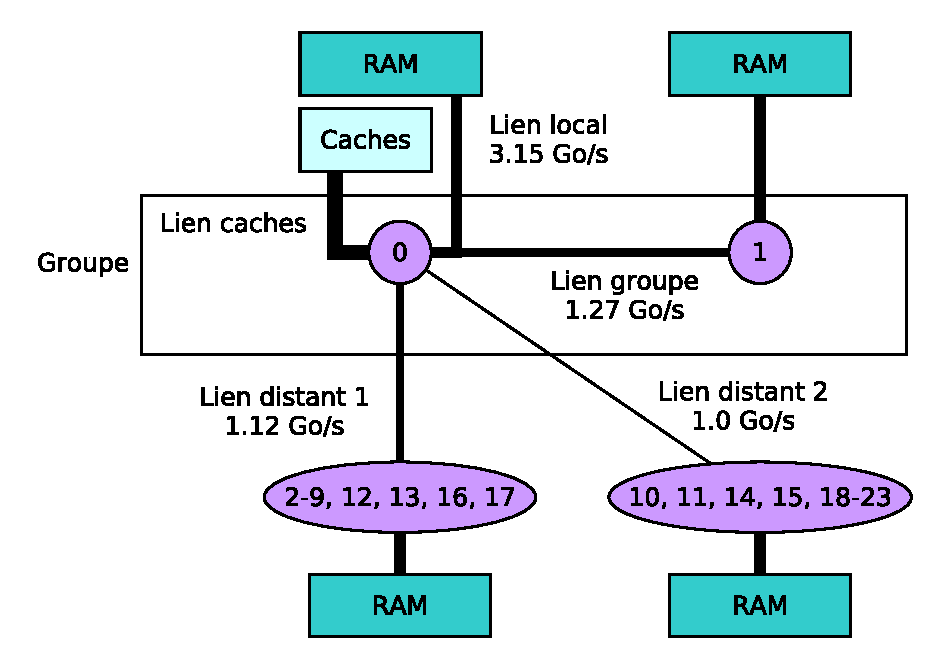
\includegraphics[width=0.8\textwidth]{topo-idchire}
  \caption{Topologie schématique vu du nœud 0}\label{fig:contribs:machines:idchire:topo-liens}
\end{figure}

L'interconnexion des nœuds NUMA est effectué à travers l'Intel \emph{Quick Path Interconnect} (QPI).
La topologie de la machine expose une hiérarchie à plusieurs niveaux, la Figure~\ref{fig:contribs:machines:idchire:topo-liens} présente la hiérarchie de la machine du point de vue du nœud 0.
Chaque nœud est d'abord associé à un autre nœud pour former un groupe. Ces groupes sont ensuite interconnectés entre eux et sont accessibles en deux rebonds maximum dans le système d'interconnexion.
Pour chaque nœud il y a 12 nœuds situés à un rebond, et 10 nœuds situés à deux rebonds.

\begin{figure}[t!]
  \centering
  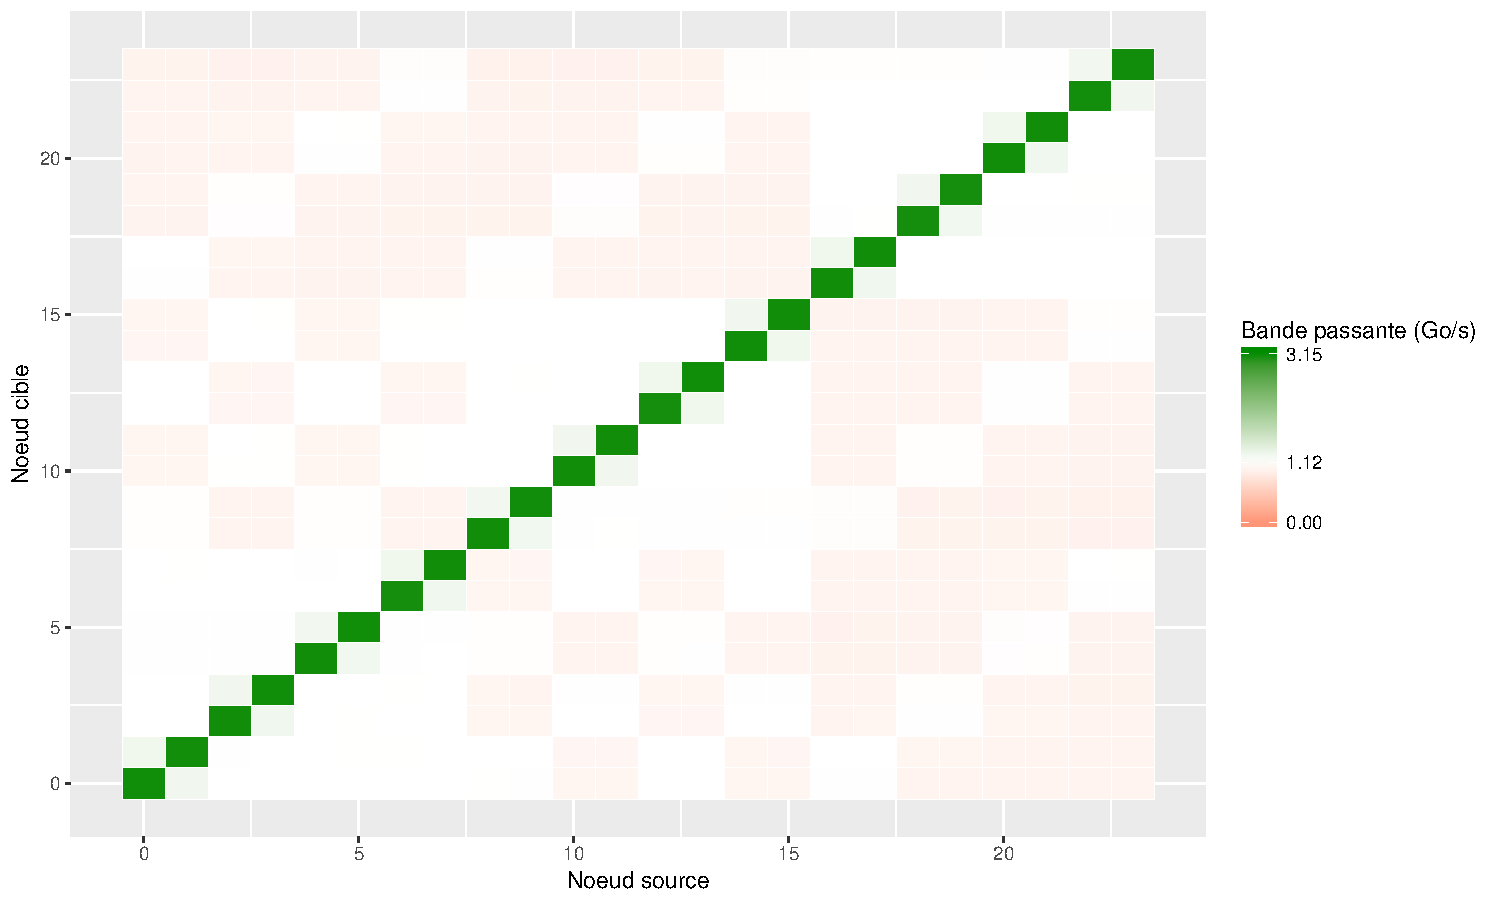
\includegraphics[width=\textwidth]{heatmap_idchire_memcpy}
  \caption{Carte de la bande passante d'idchire}\label{fig:contribs:machines:idchire:heatmap}
\end{figure}

\begin{figure}[h!]
  \centering
  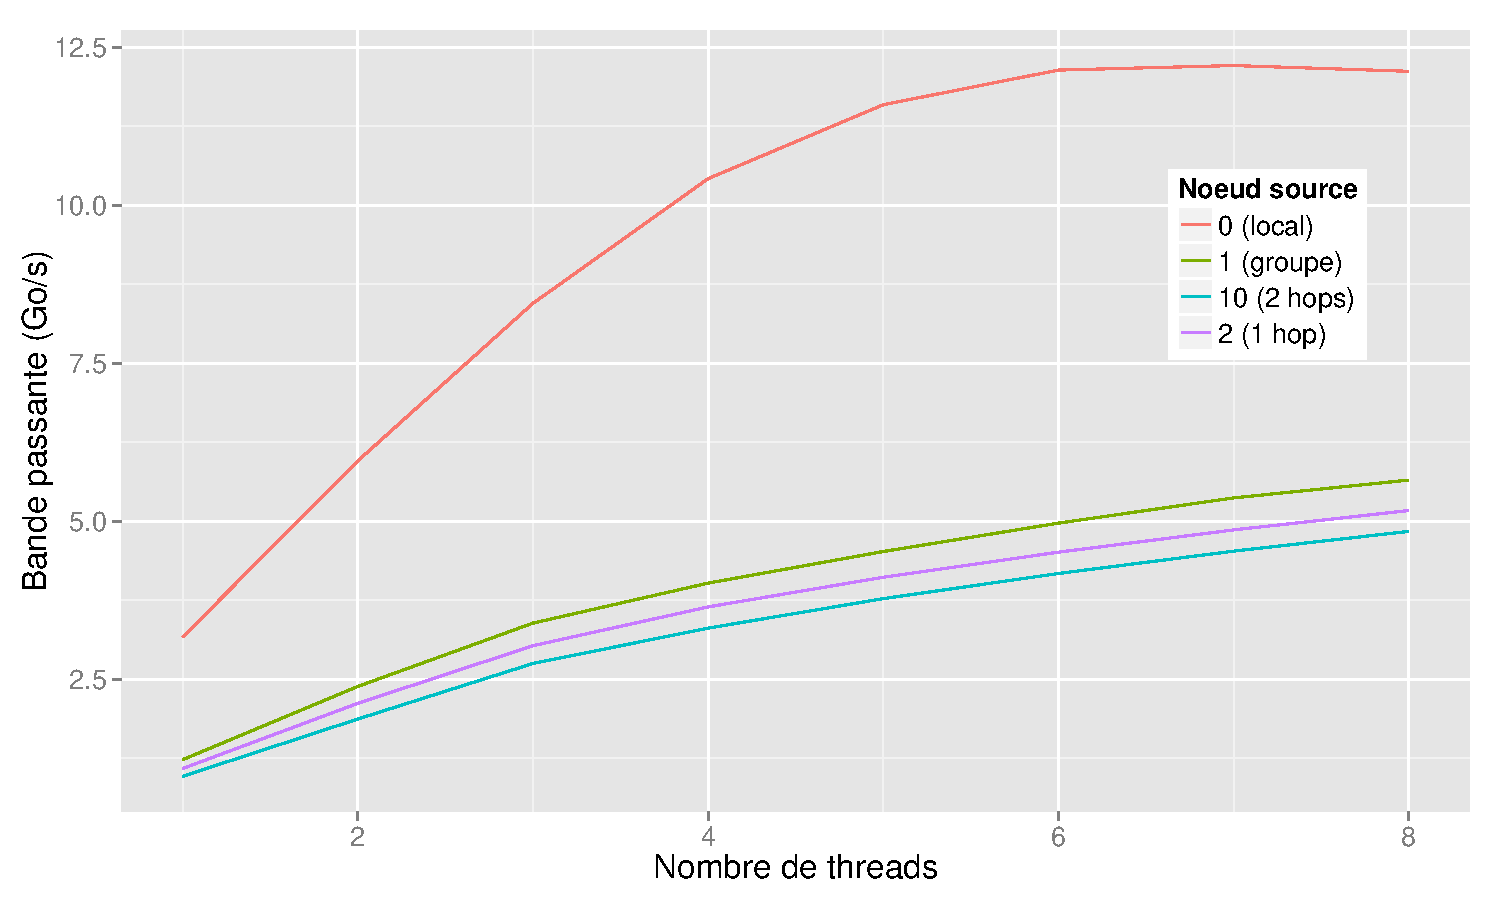
\includegraphics[width=0.9\textwidth]{link_saturation}
  \caption{Bande passante cumulée vers le nœud 0, en fonction du nombre de threads effectuant une copie et du nœud source}\label{fig:contribs:machines:idchire:saturation}
\end{figure}


La Figure~\ref{fig:contribs:machines:idchire:heatmap} présente la bande passante nœud à nœud en fonction de la source et de la destination, mesurée à l'aide d'une copie de tableau (|memcpy|) de 200 Mo.
Elle fait apparaître clairement une diagonale où la bande passante est significativement plus grande, illustrant le coût d'un accès mémoire local comparé à un accès distant.

Néanmoins cette simple <<carte>> ne suffit pas à caractériser complètement les temps d'accès aux nœuds NUMA, puisque qu'une seule communication ne va pas saturer la bande passante totale disponible, ni même illustrer l'impact de la contention.


\subsubsection{Mesure des liens}\label{sec:contribs:machines:idchire:liens}

En dehors de l'accès aux caches locaux, il y a 4 liens à quantifier, identifiés sur la Figure~\ref{fig:contribs:machines:idchire:topo-liens}.
Afin de mesurer chacun des liens, nous avons défini des scénarios spécifiques que nous avons exécuté via \outil~: pour un nœud NUMA source donné (ici 0), nous avons alloué et initialisé deux tableaux de 200 Mo. Le premier sur le nœud source, et le second sur le nœud local. Nous avons ensuite effectué une copie du tableau source vers le tableau local (via |memcpy|) et mesuré le temps de l'opération.
Pour chaque type de nœud source (même nœud, distant sur le même groupe, distant via un rebond, distant via deux rebonds), nous avons effectués de une à huit copies simultanées.


La figure~\ref{fig:contribs:machines:idchire:saturation} regroupe les résultats de la bande passante point à point, en fonction de nombre de copies simultanées ayant lieu, et en fonction du nœud d'où provient les données.
On constate que la bande passante maximum du lien local atteint 12.2 Go/s, et qu'il commence à saturer lorsque plus de la moitié des cœurs sont utilisés.
Le lien groupe plafonne à 5.6 Go/s, le lien distant 1 plafonne à 5.1 Go/s, et le lien distant 2 à 4.8 Go/s.
On peut également noter que les communications point à point sont symétriques.

\begin{figure}[ht]
  \centering
  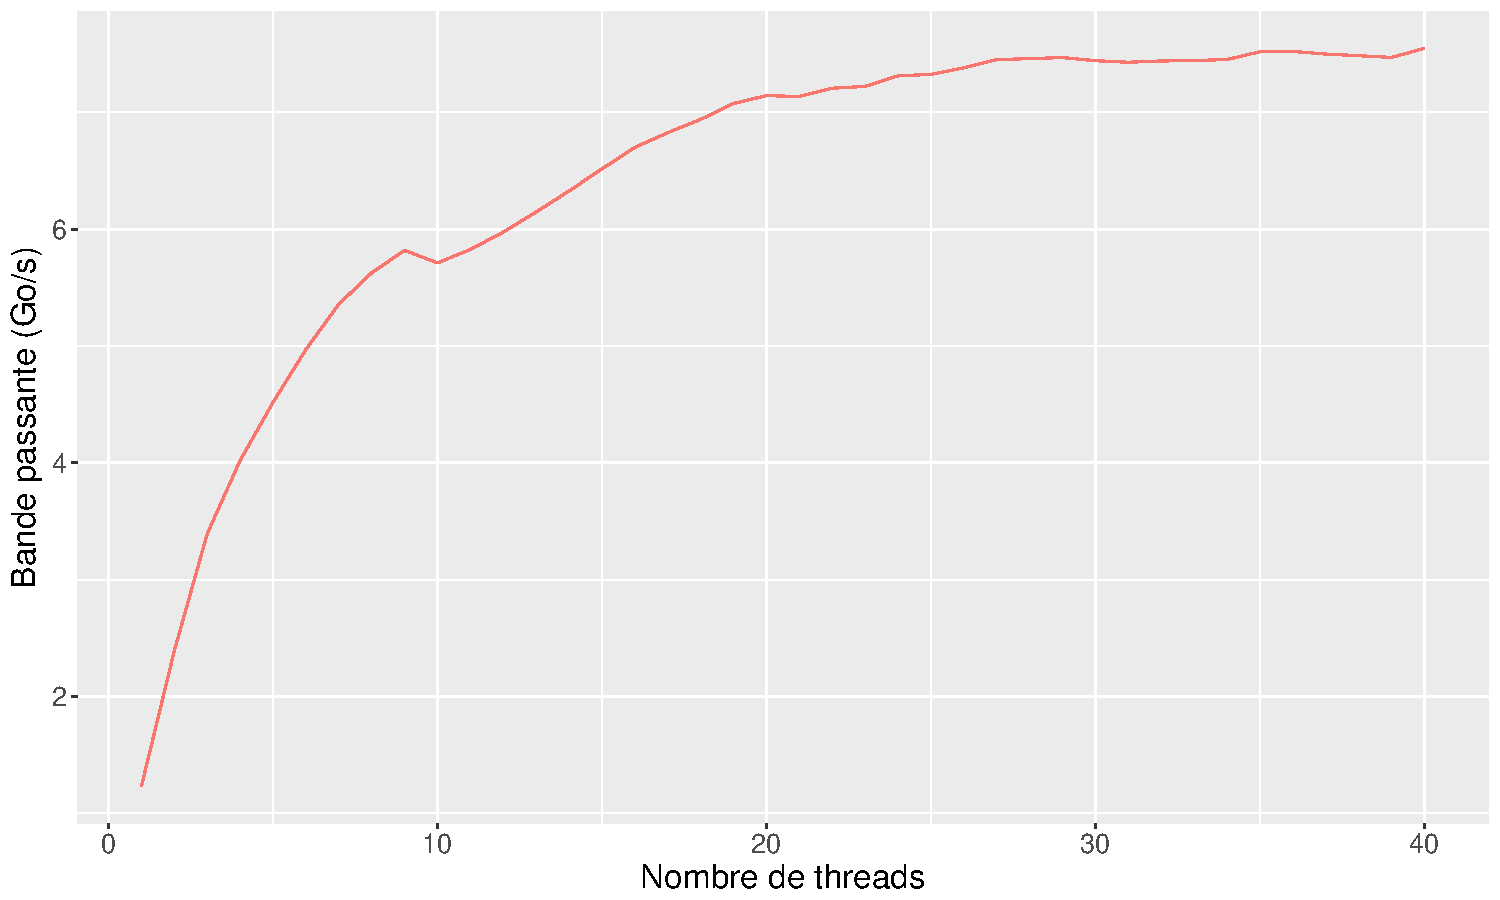
\includegraphics[width=0.9\textwidth]{link_output_saturation}
  \caption{Bande passante cumulée depuis le nœud 0 vers un nœud distant, en fonction du nombre de threads distant effectuant une copie}\label{fig:contribs:machines:idchire:saturation-output}
\end{figure}

Pour terminer la caractérisation de ces liens, nous avons finalement mesuré la bande passante maximale que l'on peut obtenir en <<sortie>> d'un nœud, en saturant les différents liens.
La figure~\ref{fig:contribs:machines:idchire:saturation-output} montre la bande passante cumulée lors d'une copie du nœud 0 vers un nœud distant, en fonction du nombre de threads effectuant une copie.
La bande passante maximale en sortie de nœud est donc de 7.5 Go/s, et commence à saturer aux alentours d'une vingtaine de copies distantes.

% TODO : si possible faire le lien saturation en sortie aussi, à voir si c'est pertinent de l'inclure


\subsection{brunch}\label{sec:contribs:machines:brunch}

Cette machine est équipée de 4 processeurs Intel(R) Xeon(R) CPU E7-8890 v4 (Broadwell), cadencés à 2.2 GHz.

Chacun de ce processeurs est associé à 378 Go de RAM pour former un nœud NUMA, ils disposent de 24 cœurs physiques partageant 60 Mo de cache L3 (20-ways associatifs).
Chacun des cœur à accès à 32 Ko de cache L1 (données) et 256 Ko de cache L2.
Les latences et bandes passantes relatives à chacun des niveaux de cache sont présentées dans le tableau~\ref{tab:synthese-processeurs}.

La machine entière dispose donc de 96 cœurs physiques, et de 1.5 To de RAM.
Les processeurs Broadwell disposent d'instructions FMA~\footnote{\emph{Fused Multiply-Add}, permettant d'effectuer une addition et une multiplication en une étape}, permettant d'effectuer 8 additions et multiplications de nombres flottant à double précision en un cycle, portant le pic de performance théorique de la machine à 3.3 TFLOPs.


\subsubsection{Topologie}

\begin{figure}[ht]
  \centering
  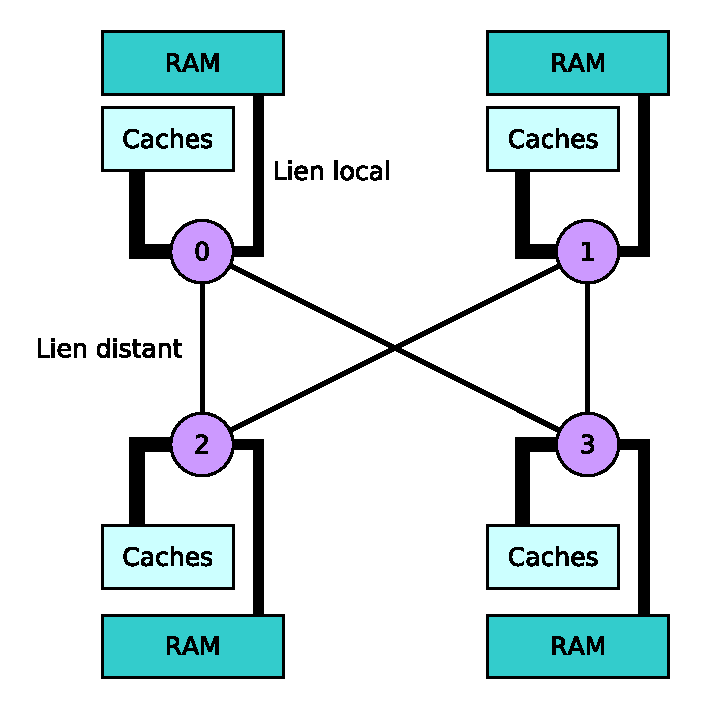
\includegraphics[width=0.6\textwidth]{topo-brunch}
  \caption{Topologie schématique complète de brunch}\label{fig:contribs:machines:brunch:topo-liens}
\end{figure}

L'interconnexion des nœuds NUMA est effectué à travers l'Intel \emph{Quick Path Interconnect} (QPI).
Contrairement à idchire, la topologie de la machine est relativement plate~: les nœuds sont directement connectés les uns aux autres, et seule la notion d'accès distant ou local permet de distinguer une hiérarchie.
La topologie complète de la machine est représentée sur la figure~\ref{fig:contribs:machines:brunch:topo-liens}

\begin{figure}[t!]
  \centering
  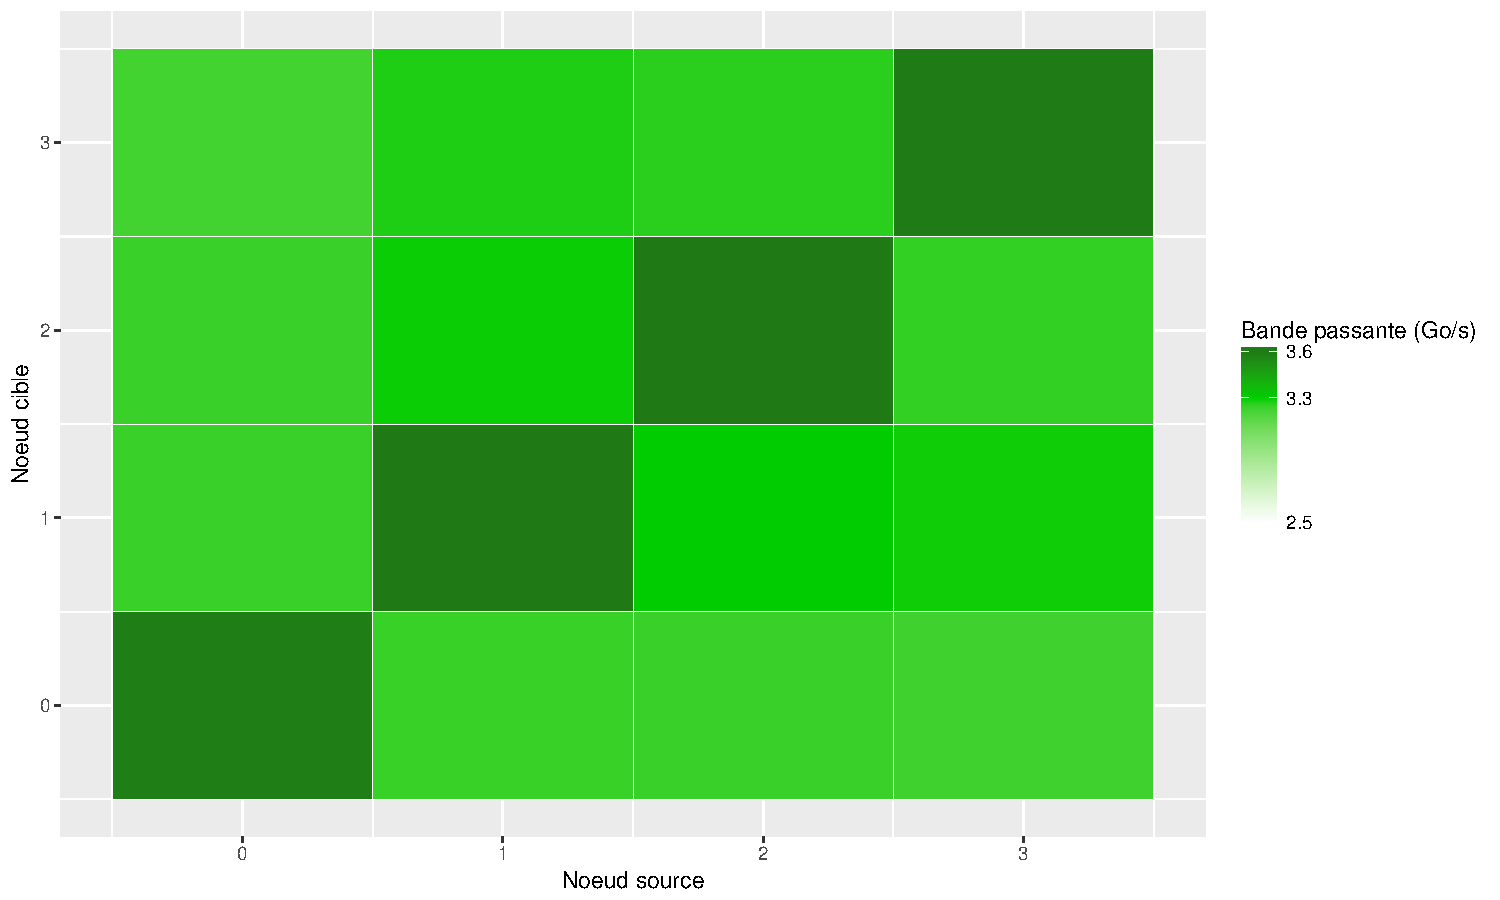
\includegraphics[width=\textwidth]{heatmap_brunch}
  \caption{Carte de la bande passante de brunch}\label{fig:contribs:machines:brunch:heatmap}
\end{figure}
\begin{figure}[h!]
  \centering
  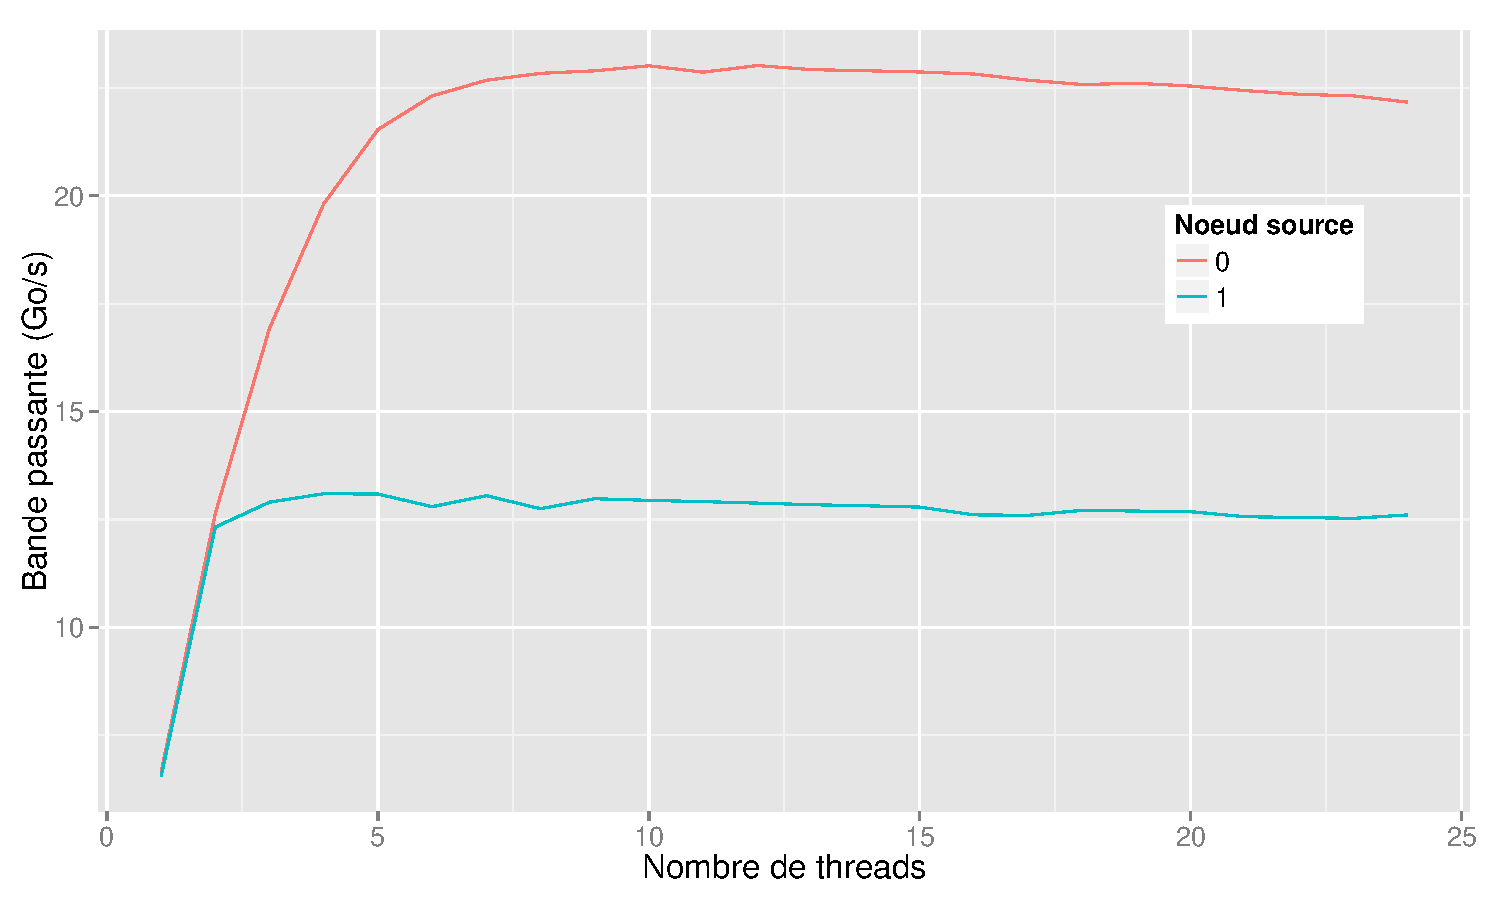
\includegraphics[width=\textwidth]{link_saturation_brunch}
  \caption{Bande passante cumulée depuis le nœud 0, en fonction du nombre de threads effectuant une copie et du nœud destination}\label{fig:contribs:machines:brunch:saturation}
\end{figure}


La Figure~\ref{fig:contribs:machines:brunch:heatmap} présente la bande passante nœud à nœud en fonction de la source et de la destination, mesurée à l'aide d'une copie de tableau (|memcpy|) de 200 Mo.
Bien qu'une diagonale se dégage clairement, la différence entre accès local et accès distant n'est de l'ordre que de 10\%, comme en témoigne l'échelle de couleur sur la figure.

\subsubsection{Mesure des liens}

De même que pour idchire, nous avons effectué des observations complémentaires pour caractériser plus précisément les liens locaux et distant, afin de déterminer leur saturation.
Les résultats de ces expériences ont été rassemblés sur la figure~\ref{fig:contribs:machines:brunch:saturation}.
Bien que la bande passante soit bien plus importante que sur idchire, les liens arrivent à saturation bien plus vite~: à peine 20\% de charge du nœud permet de saturer la bande passante.

\bigskip
\bigskip

Ces résultats sur les capacités physique des machines vont avoir un impact important dans la section suivante~: nous allons faire une étude de cas d'une application - la factorisation de Cholesky, et nous allons en étudier individuellement les parties critiques.
Certaines de ces parties critiques peuvent utiliser un large ensemble de données, en pleine charge de la machine les performances seront donc limitées par les résultats que nous venons de décrire.


\section{Une étude de cas : Cholesky}\label{sec:contribs:apps:cholesky}

Afin de mettre en application nos analyses nous avons choisi comme cas d'étude une application d'algèbre linéaire populaire et bien connue : la factorisation de Cholesky.
Une manière standard de paralléliser les applications d'algèbre linéaire est de découper le problème en l'appliquant à différentes sous parties (ou \emph{blocs}) des matrices.

Nous allons étudier en détails l'algorithme de Cholesky par bloc, voir quelles sont ses parties critiques et leurs comportements, et nous allons également voir comment nous avons pu améliorer son exécution.


\subsection{Description générale}

La factorisation de Cholesky a pour but de résoudre l'équation suivante :

$$ A = L*L^T$$

Où $A$ est une matrice symétrique définie positive de nombre réels, et $L$ est l'inconnue, une matrice triangulaire inférieure.

Pour paralléliser la résolution de cette équation, on va découper la matrice $A$ par bloc, et appliquer un algorithme de Cholesky par bloc.
On peut donc caractériser une factorisation de Cholesky par sa taille de bloc et sa largeur en nombre de blocs.

L'algorithme de résolution par bloc repose sur quatre algorithmes basiques d'algèbre linéaire tirés des \emph{BLAS} - \emph{Basic Linear Algebra Subprograms} - décrit ci-dessous~:


\paragraph{\potrfcolor{POTRF(A)}}

Ce noyau effectue la factorisation de Cholesky de base sur une matrice $A$.

\paragraph{\trsmcolor{TRSM(A, B)}}

Ce noyau effectue l'opération suivante~: $A*X = B$, où $A$ est une matrice triangulaire, et $B$ une matrice générique. $B$ est écrasée par la matrice solution $X$.

\paragraph{\syrkcolor{SYRK(A, C)}}

Ce noyau effectue l'opération suivante~: $C = A*A' + C$, où $A$ est une matrice générique, et $C$ est une matrice symétrique.

\paragraph{\gemmcolor{GEMM(A, B, C)}}

Ce noyau effectue une multiplication de matrices génériques, définie de la manière suivante~: $C = A*B + C$, où $A$, $B$, et $C$ sont des matrices génériques.

\begin{figure}[h]
  \centering
  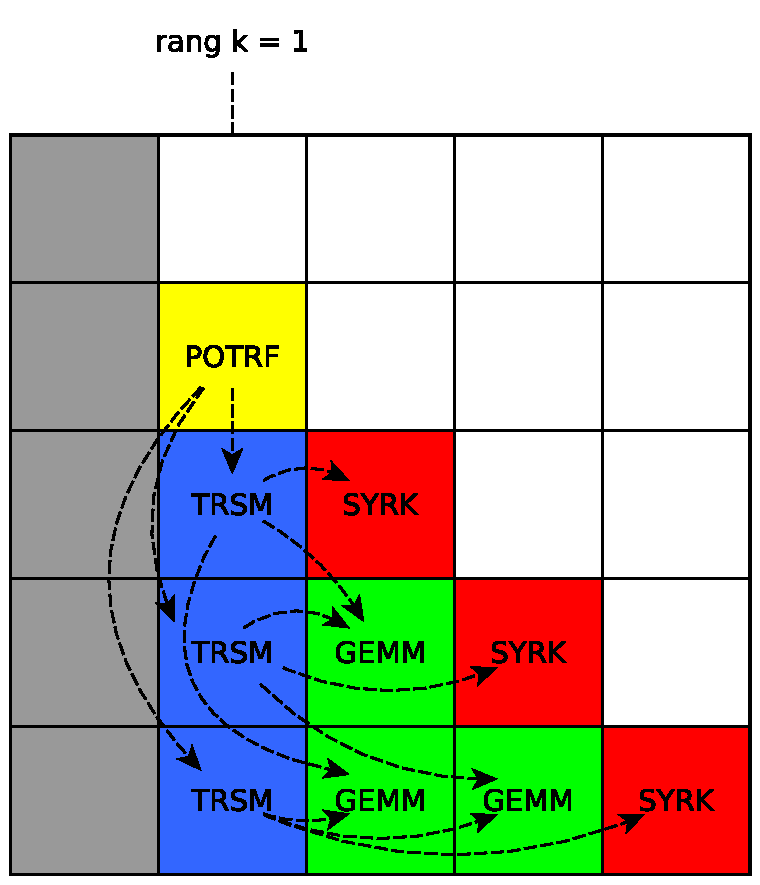
\includegraphics[width=0.6\textwidth]{cholesky-rank-update}
  \caption{Itération du rang k de la factorisation de Cholesky}\label{fig:contribs:apps:cholesky:rank-update}
\end{figure}

\paragraph{L'algorithme par bloc}

L'algorithme peut se formuler de la manière suivante~:

\begin{lstlisting}[language=c++]
for (int k = 0; k < n_blocs; k++) {
  DPOTRF(A(k, k));

  for (int m = k+1; m < n_blocs; m++) {
    DTRSM(A(k, k), A(k, m));

    for (int m = k+1; m < n_blocs; m++) {
      DSYRK(A(k, m), A(k, k));

      for (int n = k+1; n < m; n++) {
        DGEMM(A(k, n), A(k, m), A(n, m));
      }
    }
  }
}
\end{lstlisting}

Pour permettre de mieux représenter l'algorithme, les opérations se produisant sur chaque bloc de la matrice au rang |k| sont illustrées sur la figure~\ref{fig:contribs:apps:cholesky:rank-update}


À chaque itération, un \potrf est d'abord effectué sur le bloc diagonal de l'itération. Les blocs de la colonne sont ensuite mis à jour via des \trsm, à la suite desquels les autres blocs restant peuvent être mis à jour par des \gemm (ou \syrk pour les blocs diagonaux).
Le parallélisme de l'algorithme est donc principalement libéré par les \potrf ainsi que les \trsm.

Cela peut être illustré par la Figure~\ref{fig:contribs:apps:cholesky:dag-5}, qui donne le graphe de dépendances d'une factorisation de Cholesky de largeur 5.
Le chemin critique de l'application est mis en valeur avec des liens en gras. Comme on peut le constater, tous les \potrf se trouvent sur ce chemin critique.

\begin{figure}[h]
  \centering
  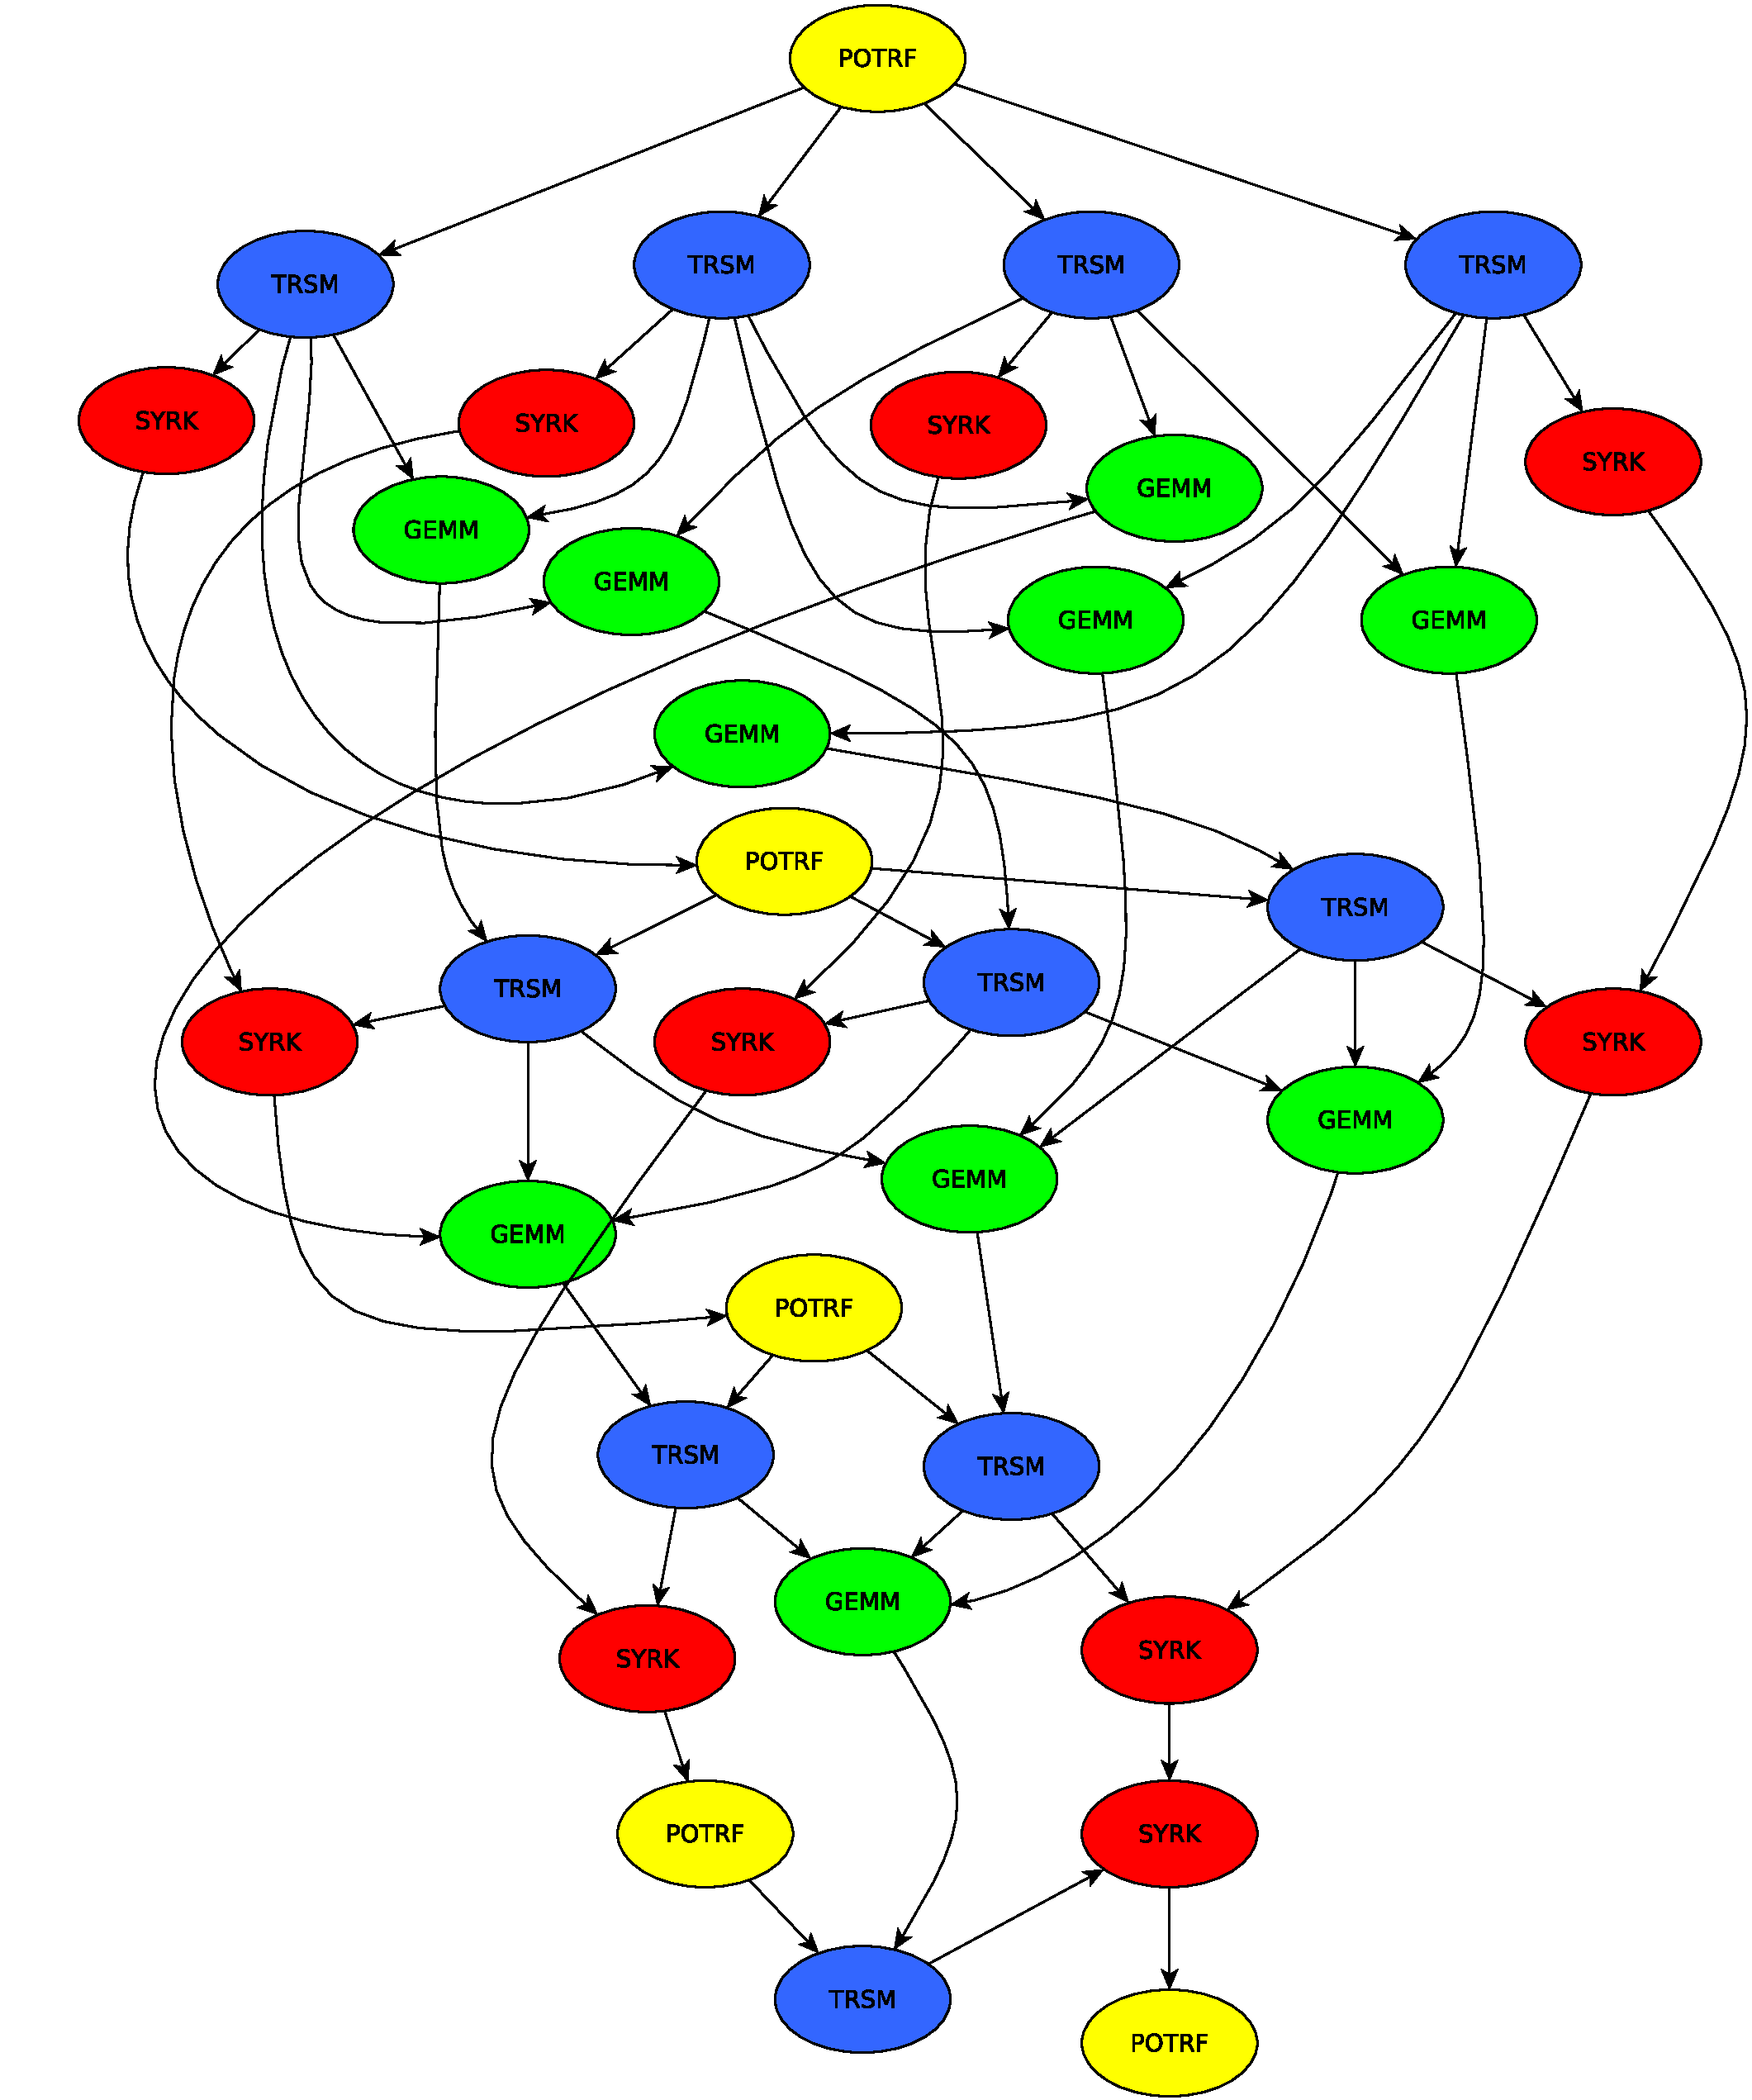
\includegraphics[width=0.7\textwidth]{cholesky-dag-5}
  \caption{DAG d'un Cholesky de largeur 5}\label{fig:contribs:apps:cholesky:dag-5}
\end{figure}

Le nombre de tâches créées au rang $k$, ainsi que le nombre d'opérations arithmétiques, ou \emph{flops}, sont résumés dans la table~\ref{tab:contribs:apps:cholesky:kernels-info}.

\begin{table}[h]
\def\arraystretch{1.5}
\centering
\begin{tabular}{|c||c|c|}\hline
  Noyau & Nombre au rang $k$ & Flops en fonction de la taille de bloc $N$~\cite{LAWN41} \\ \hline
  \potrf & 1 & $\frac{N^3}{3} + \frac{N^2}{2} + \frac{N}{6}$ \\ \hline
  \trsm & $k$ & $N^3$ \\ \hline
  \syrk & $k$ & $N^2*(N+1)$ \\ \hline
  \gemm & $\frac{k*(k-1)}{2}$ & $2*N^3$ \\ \hline
\end{tabular}
\caption{Nombre et complexité des différents noyaux}\label{tab:contribs:apps:cholesky:kernels-info}
\end{table}

Les \gemm sont donc très largement majoritaires dans l'algorithme quand la largeur de la matrice augmente, et sont également les plus intensifs en terme d'opérations.

\subsection{Observations préliminaires et limites}

La figure~\ref{fig:context:granularity} a montré qu'on pouvait observé l'impact de certains paramètres, tels que la taille de bloc ou le support exécutif, sur les performances globales.

Certains supports exécutifs permettent d'aller plus loin via un système de traces, permettant d'observer certaines caractéristiques de tâches particulières.

\begin{figure}[t!]
  \centering
  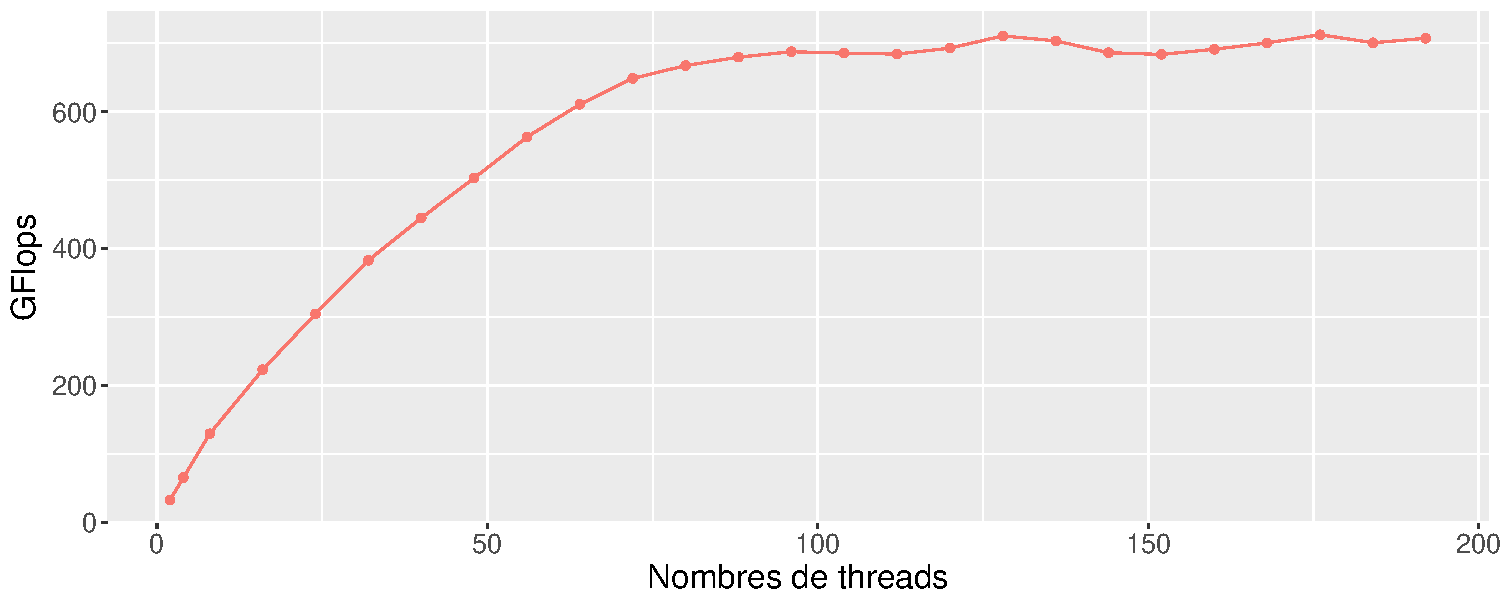
\includegraphics[width=\textwidth]{graph_evolution_cholesky_8192_224}
  \caption{Évolution des performances de Cholesky pour une taille de matrice de 8192 et une taille de bloc de 224}\label{fig:contribs:apps:cholesky:overview-8192-224}
\end{figure}

Pour illustrer cela, prenons un exemple d'évolution des performances de Cholesky en fonction du nombre de cœurs utilisés, montré sur la figure~\ref{fig:contribs:apps:cholesky:overview-8192-224}. Dans cette exemple la taille de matrice est de 8192, la taille de bloc de 224, et le support exécutif utilisé est libKOMP.

En activant le support des traces, on peut avoir plus de détails sur l'exécution individuelle de chacune des tâches.

\begin{figure}[h!]
  \centering
  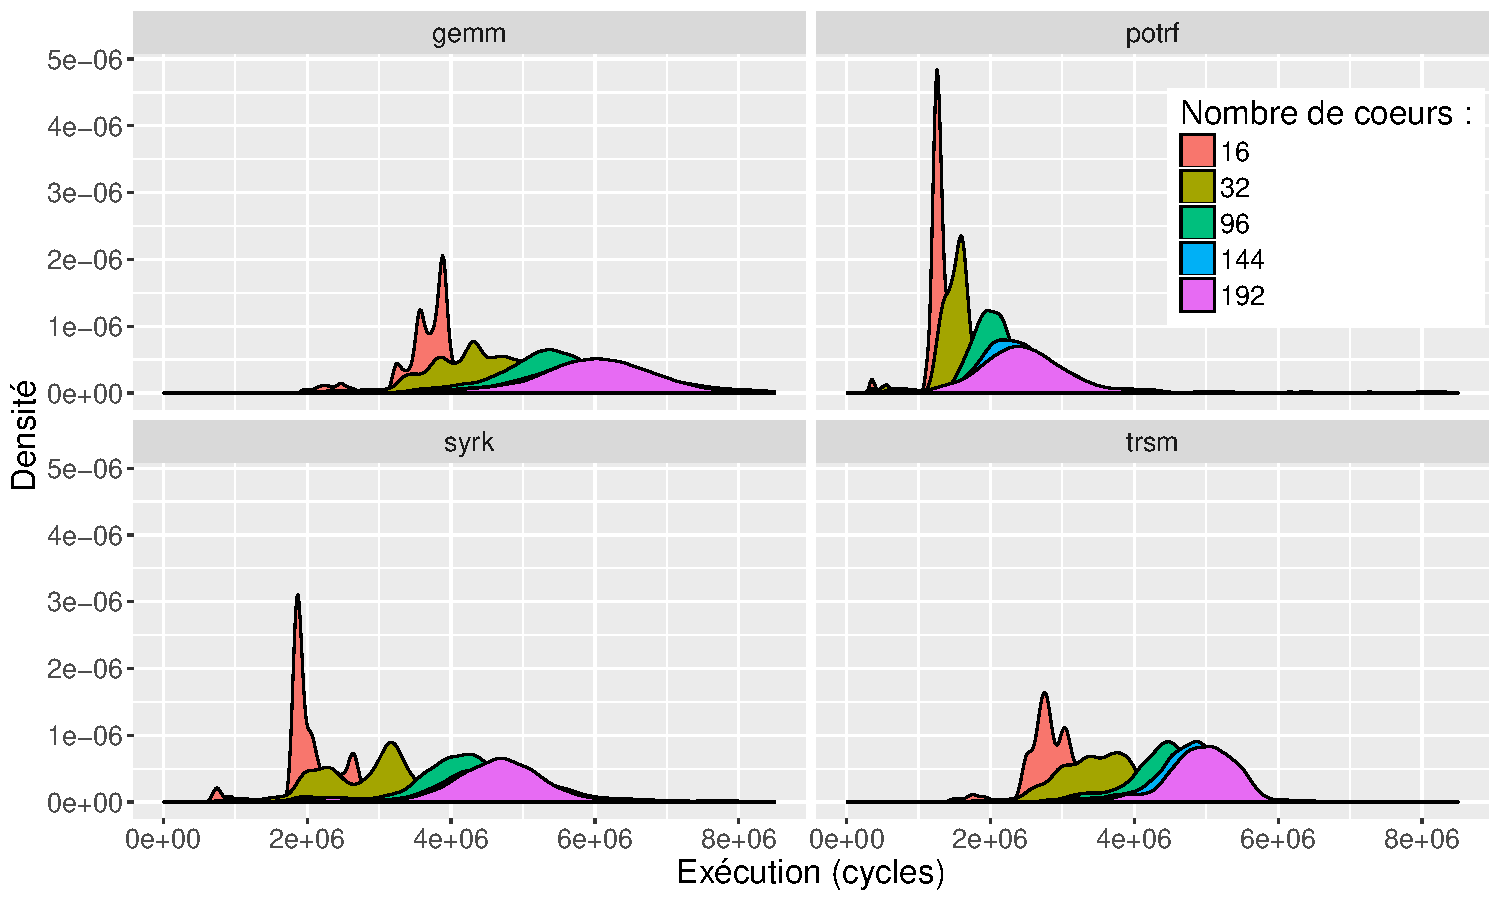
\includegraphics[width=\textwidth]{graph_distrib_overview_8192_224}
  \caption{Distribution des différents noyaux en fonction du nombre de cœurs}\label{fig:contribs:apps:cholesky:distrib-overview-8192-224}
\end{figure}

La figure~\ref{fig:contribs:apps:cholesky:distrib-overview-8192-224} montre, pour chaque type de tâche (ou \emph{noyau}), la répartition du temps d'exécution (en cycles) en fonction du nombre de cœurs.

À part pour 16 cœurs, on peut constater que la répartition est assez large~: pour un \gemm sur 192 cœurs, le nombre de cycles nécessaire pour l'exécution peut varier du simple au double !
Nous souhaiterions donc identifier d'où vient ce phénomène, afin d'éventuellement le corriger, et retomber sur un pic de performance clair et stable (comme par exemple pour la distribution des \potrf sur 16 cœurs).

Malheureusement il n'existait pas, à notre connaissance, d'outil permettant d'isoler une (ou plusieurs) tâches d'une application, et permettant de changer certains paramètres prédéfinis pouvant avoir un impact sur le temps d'exécution de la tâche.
Nous avons donc utilisé \outil dans le but de comprendre et d'analyser plus en profondeur nos observations préliminaires.

\subsection{Caractérisation détaillée des noyaux via \outil}

L'objectif de cette section est de décrire le processus expérimental nous ayant permis d'analyser et comprendre le comportement des quatre noyaux de Cholesky~: \potrf, \trsm, \syrk, \gemm, qui a finalement abouti à des améliorations du support exécutif.
Nous allons donc aborder d'une part les types de scénarios exécutés via \outil, puis illustrer les résultats que nous avons obtenus avec des exemples significatifs.

\subsubsection{Description des scénario}

Afin d'étudier le comportement de chaque noyau impliqué dans Cholesky, nous avons définie des scénerios où ils sont exécutés avec un contrôle sur les conditions d'exécution.

Pour un noyaux donné (parmi \potrf, \trsm, \syrk, \gemm), le scénario de base est le suivant :
\begin{itemize}
  \item Allocation et initialisation des données sur un nœud précis.
  \item Exécution d'un certain nombre de répétitions du noyau choisi (par défaut 50), soit sur un cœur du même nœud, soit sur un cœur distant, pour une taille de bloc donnée.
  \item Observation de la performance en FLOPS.
\end{itemize}

Pour évaluer le comportement des noyaux en fonction de la charge de la machine, nous avons créé des scénarios exécutant plusieurs scenarios de base, de manière indépendante, et où le démarrage de l'exécution des noyaux est synchronisé.

Il y a donc plusieurs paramètres que l'on peut faire varier pour changer les conditions d'exécution~:
\begin{itemize}
  \item Le nombre de noyaux s'exécutant simultanément
  \item L'utilisation de données distantes ou locales
  \item La taille du bloc sur lequel appliquer le noyau
\end{itemize}

Les trois sections suivantes décrivent l'impact des changements de ces paramètres, et illustrent certaines caractéristiques des machines utilisées qui donnent des opportunités pour de possibles améliorations du support exécutif.

\subsubsection{Exécutions concurrentes}

\begin{figure}[ht]
  \centering
  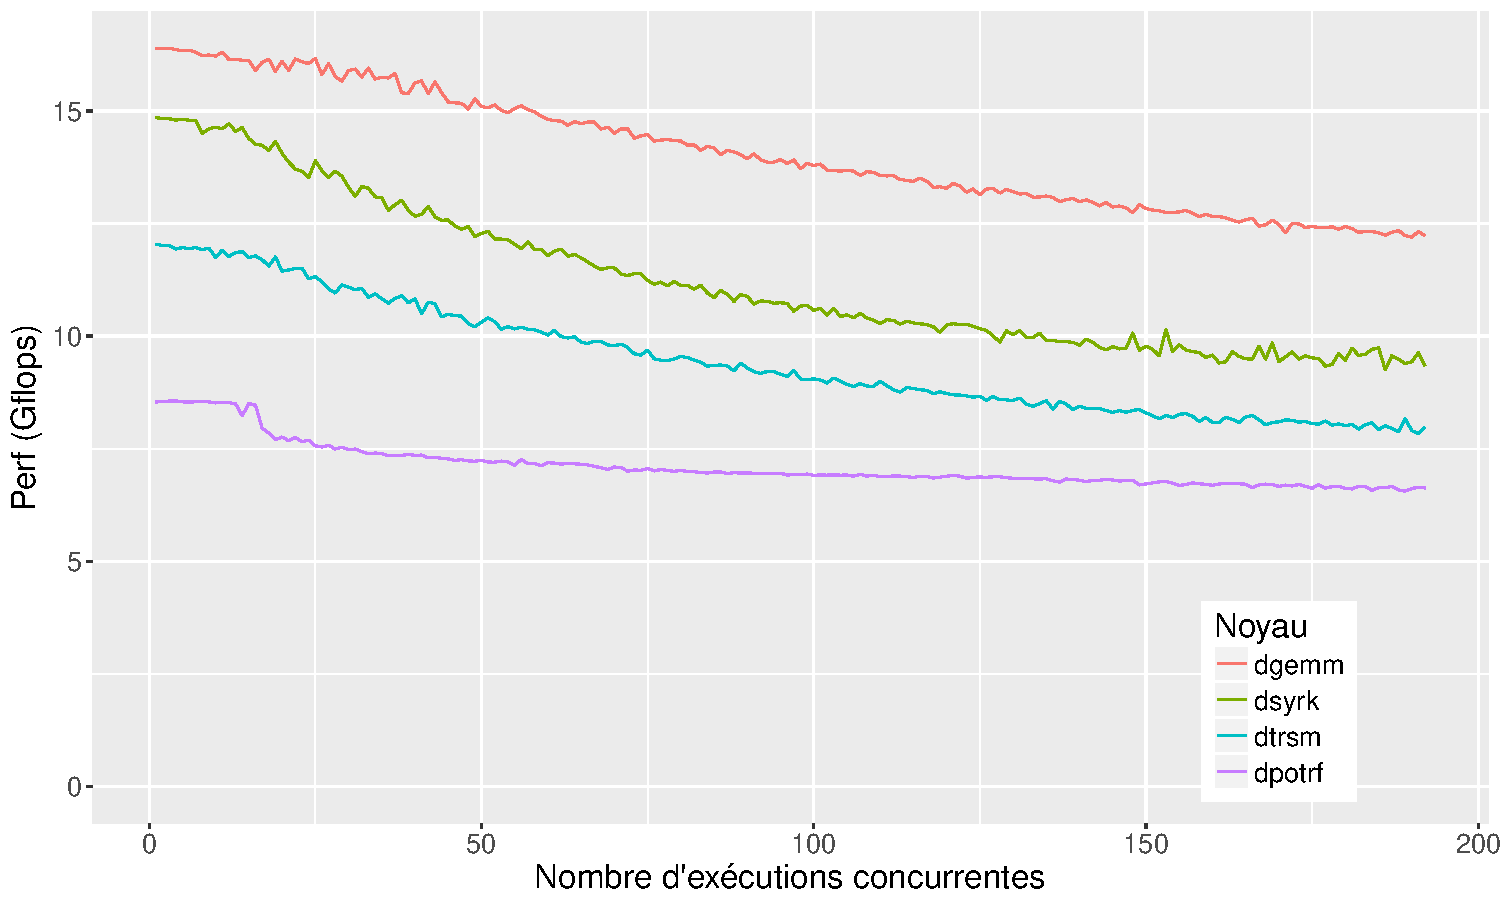
\includegraphics[width=0.95\textwidth]{kernel_256_local_idchire}
  \caption{Performances des noyaux (B=256) avec données locales sur idchire}\label{fig:contribs:apps:cholesky:perf-256-local}
\end{figure}

Afin d'évaluer l'impact de la charge de la machine, nous avons lancé des scénarios avec un nombre variable d'exécution concurrentes de chacun des noyaux. La figure~\ref{fig:contribs:apps:cholesky:perf-256-local} montre la performance moyenne (en GFlops) de chaque noyau, en fonction du nombre de cœurs exécutant des noyaux en concurrence.
Par exemple pour déterminer le point d'abscisse 150 sur la figure pour un \gemm, nous avons exécuté 50 répétitions de \gemm sur chacun des 150 premiers cœurs de la machine idchire, de manière indépendante et concurrente.
La performance moyenne pour ce point est obtenue en faisant la moyenne des performances sur l'ensemble des exécutions.
Pour ce cas la taille de bloc a été fixée à 256, avec les données allouées et initialisées localement.

Pour une taille de bloc de 256, la quantité maximale de données utilisée par l'un des noyaux (\gemm) est de 256*256*8*3 = 1.5 Mo. Avec un nœud de 8 cœurs exécutant 8 exécutions concurrentes, la quantité totale de données utilisée serait au pire de 12.58 Mo, soit environ 50\% des 20Mo de cache L3 disponible.
On pourrait donc s'attendre à ce que la performance moyenne des noyaux ne soit impactés que par des effets locaux aux nœuds.

Néanmoins les courbes montrent clairement une dégradation des performances de chaque noyaux lorsque la charge de la machine augmente.
Ce comportement a également été observé pour d'autres tailles de blocs. Sur brunch le comportement a été également observé, avec une dégradation moindre néanmoins.

\begin{todo}
  ici l'explication est toujours pas évidente : certes le nombre de messages broadcasté dépend de la quantité de données utilisées (cf lien en commentaire), mais la source principale de comm c'est les miss au L3.
  
  Là on a que des miss au L2, ça implique un write-back au L3, mais est-ce suffisant pour expliquer le phénomène ?
  %https://www.researchgate.net/profile/Daniel_Molka/publication/315703632_Performance_Analysis_of_Complex_Shared_Memory_Systems/links/58dd3cf292851cd2d3d9d5d3/Performance-Analysis-of-Complex-Shared-Memory-Systems.pdf
  %https://pdfs.semanticscholar.org/67cf/1189c859d66bac309f9438df434fb651f97a.pdf
  % sandy bridge : https://tu-dresden.de/zih/forschung/ressourcen/dateien/abgeschlossene-projekte/benchit/2014_MSPC_authors_version.pdf?lang=en
  % haswell : https://pdfs.semanticscholar.org/67cf/1189c859d66bac309f9438df434fb651f97a.pdf
\end{todo}

\subsubsection{Impact de la localité des accès}

La section~\ref{sec:contribs:machines} a montré des différences significatives dans les temps d'accès à la mémoire locale et distante.
Nous avons donc déroulé des scénarios avec des noyaux utilisant des données distantes ou des données locales afin de pouvoir les comparer, et éventuellement déceler des comportements typiques.

\begin{figure}[t!]
  \centering
  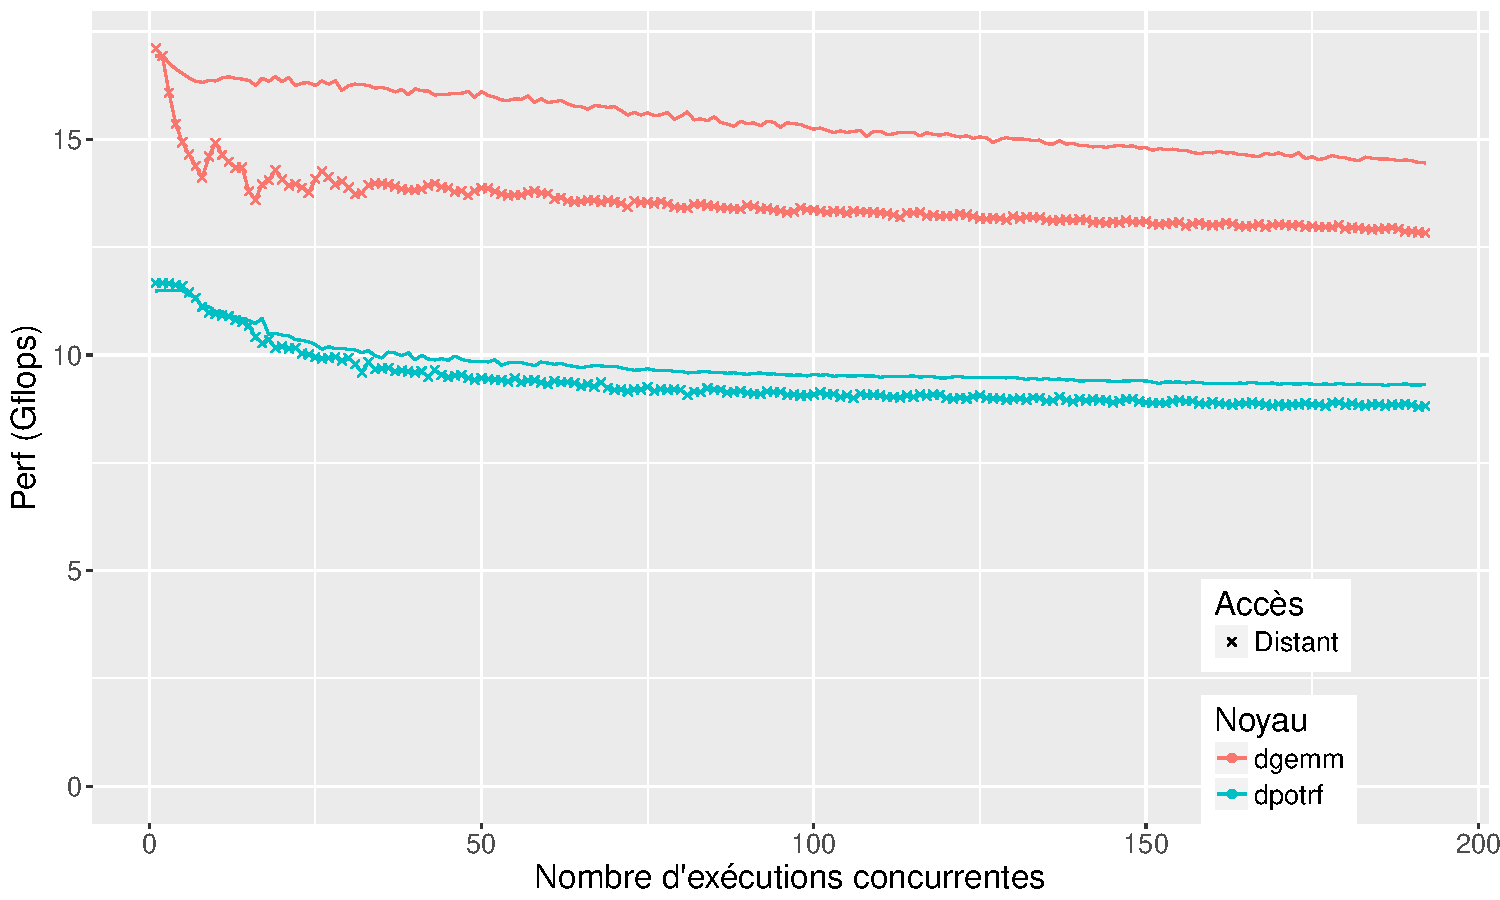
\includegraphics[width=0.95\textwidth]{kernel_512_remote_idchire}
  \caption{Performances GEMM, POTRF (B=512) avec données distantes sur idchire}\label{fig:contribs:apps:cholesky:perf-512-remote-idchire}
\end{figure}
\begin{figure}[h!]
  \centering
  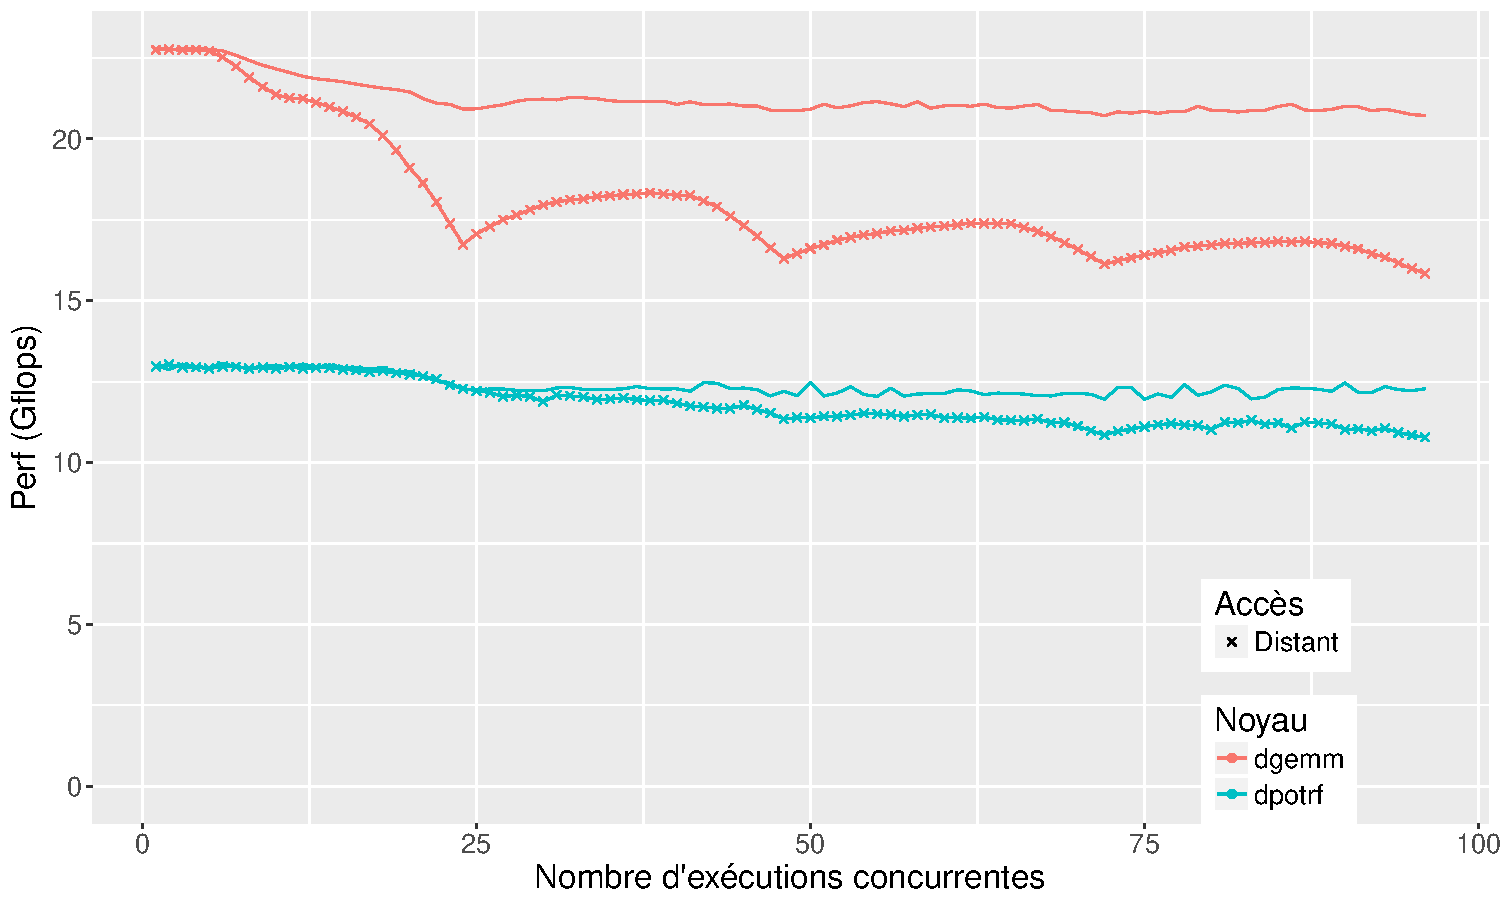
\includegraphics[width=0.95\textwidth]{kernel_512_remote_brunch}
  \caption{Performances GEMM, POTRF (B=512) avec données distantes sur brunch}\label{fig:contribs:apps:cholesky:perf-512-remote-brunch}
\end{figure}

Les figures~\ref{fig:contribs:apps:cholesky:perf-512-remote-idchire} et~\ref{fig:contribs:apps:cholesky:perf-512-remote-brunch} illustrent les performances de deux noyaux, \gemm et \potrf, effectués en concurrence sur des blocs de 512, en fonction du type d'accès, sur idchire et brunch, respectivement.

Avec une telle taille de bloc, l'ensemble des données pour tous les \potrf tient dans le cache L3, mais ce n'est pas le cas pour \gemm.
Pour les \potrf la dégradation de performances est moindre : les données tiennent dans le cache L3, il y a donc un coup pour rapatrier les données, mais une fois les données dans le cache L3 il n'y a plus besoin de faire d'accès distants.

Pour les \gemm, une utilisation de seulement quelques cœurs ne montre pas une différence de performances flagrante, en revanche le lien en sortie de nœud arrive assez vite à saturation (voir section~\ref{sec:contribs:machines:idchire:liens}), ce qui entraine une dégradation massive de performances.
À la fois pour idchire et brunch, on peut observer l'impact de la bande passante sur les performances : les courbes sont en dent de scie avec une période égale à la taille des nœuds sur chaque machine (8 sur idchire, 24 sur brunch).

Cela devient évident lorsqu'on regarde plus en détail le passage d'un nœud à un autre.
Sur la figure~\ref{fig:contribs:apps:cholesky:perf-512-remote-brunch}, la courbe pour les \gemm distants remonte progressivement entre 24 et 36 cœurs utilisés~: le fait de faire la moyenne des noyaux sur l'ensemble des cœurs cache légèrement le phénomène de saturation du lien.
En revanche ce phénomène devient évident lorsque l'on affiche la moyenne du temps d'exécution par cœurs pour certains des points de la courbe, comme illustré sur la figure~\ref{fig:contribs:apps:cholesky:distrib-load-512}.

\begin{figure}[ht]
  \centering
  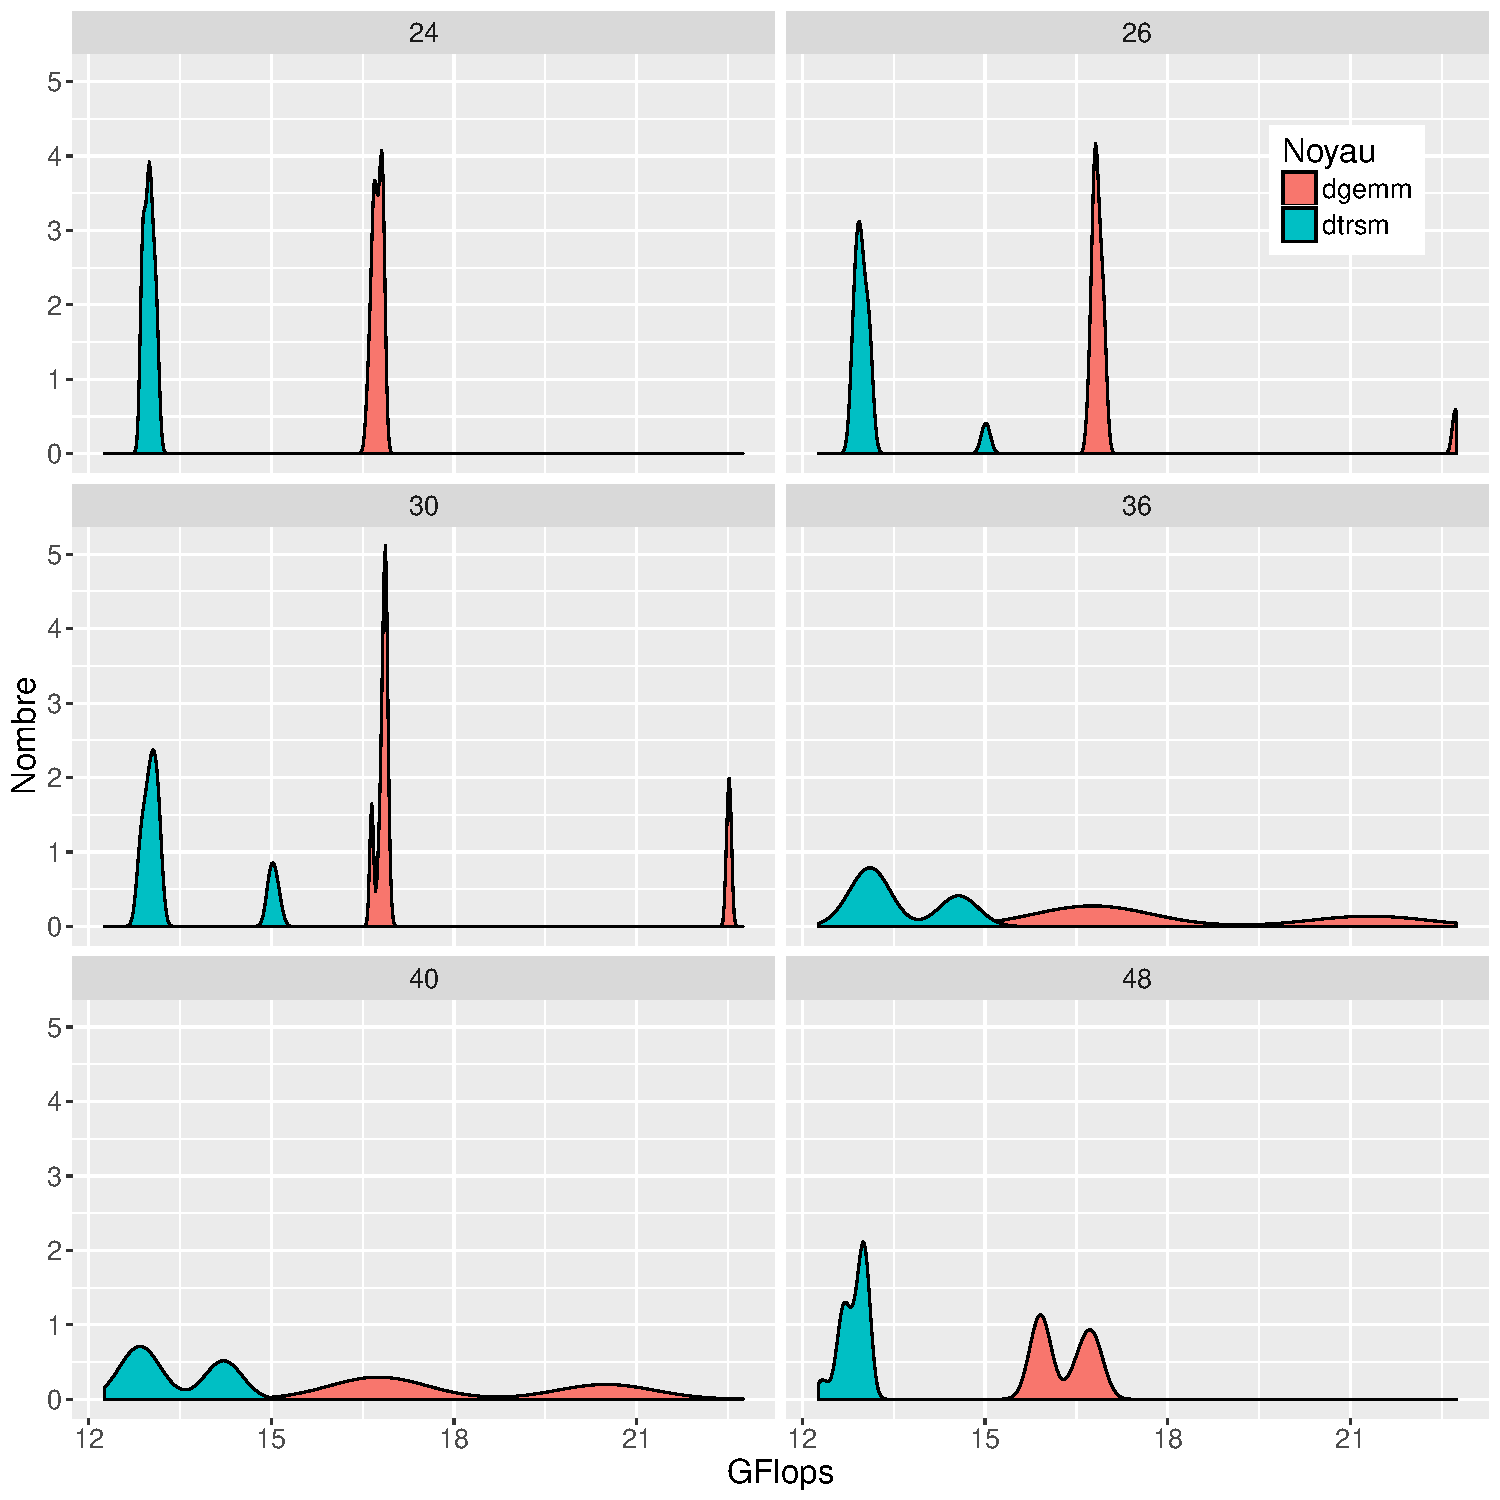
\includegraphics[width=0.95\textwidth]{illustration_load_avg}
  \caption{Distribution des performances de chaque noyau (Bloc = 512), en fonction du nombre total d'exécutions concurrentes, sur brunch}\label{fig:contribs:apps:cholesky:distrib-load-512}
\end{figure}

Le premier panneau montre la distribution des \gemm et des \potrf pour une exécution sur 24 cœurs concurrents situés sur le même nœuds.
Cette distribution montre un unique pic bien définie pour chaque noyau (environ 13 GFlops pour \potrf, et 16.5 pour \gemm).
En revanche le passage à 26 cœurs (avec donc 2 cœurs situés seuls sur un autre nœud), montre une distribution avec deux pics~: un pic important correspondant au 24 premiers cœurs, et un second pic plus petit, montrant des performances beaucoup plus grandes, pour les 2 cœurs situé sur l'autre nœud.
Les autres panneaux montrent l'évolution de ces pics pour arriver au panneau 48, où les deux nœuds sont complètement utilisés.

\begin{todo}
  Ici il y a aussi deux pics sur le panneau 48. Cela doit venir de la manière dont j'ai initialisé les accès distants : le premier nœud utilise des données du deuxième nœud, qui utilise des données du troisième nœud. Donc en pratique les liens du deuxième nœuds sont plus utilisés que ceux du premier : il doit donc un peu peiner à fournir les données nécessaires au premier nœud, ce qui expliquerait pourquoi il y a deux groupes de perf.
\end{todo}


L'impact de la localité des données est majeure dans le cas où le jeu de données manipulé par l'ensemble des cœurs ne tient pas dans le cache L3.
Étant donné que la plus grande proportion des noyaux de Cholesky manipule 2 ou 3 blocs, la dégradation de performance devrait être importante lorsque la taille de bloc dépasse environ 320.

% Note : à la fois sur brunch et idchire, chaque cœur peut utiliser environ 2.5Mo de cache L3



\subsubsection{Impact de la taille de bloc}

La figure~\ref{fig:contribs:apps:cholesky:perf-multiple-bs-idchire} montre la performance des \gemm et \potrf sur idchire en fonction de la taille de bloc et du nombre de cœurs utilisés (tous les accès sont locaux).

\begin{figure}[ht]
  \centering
  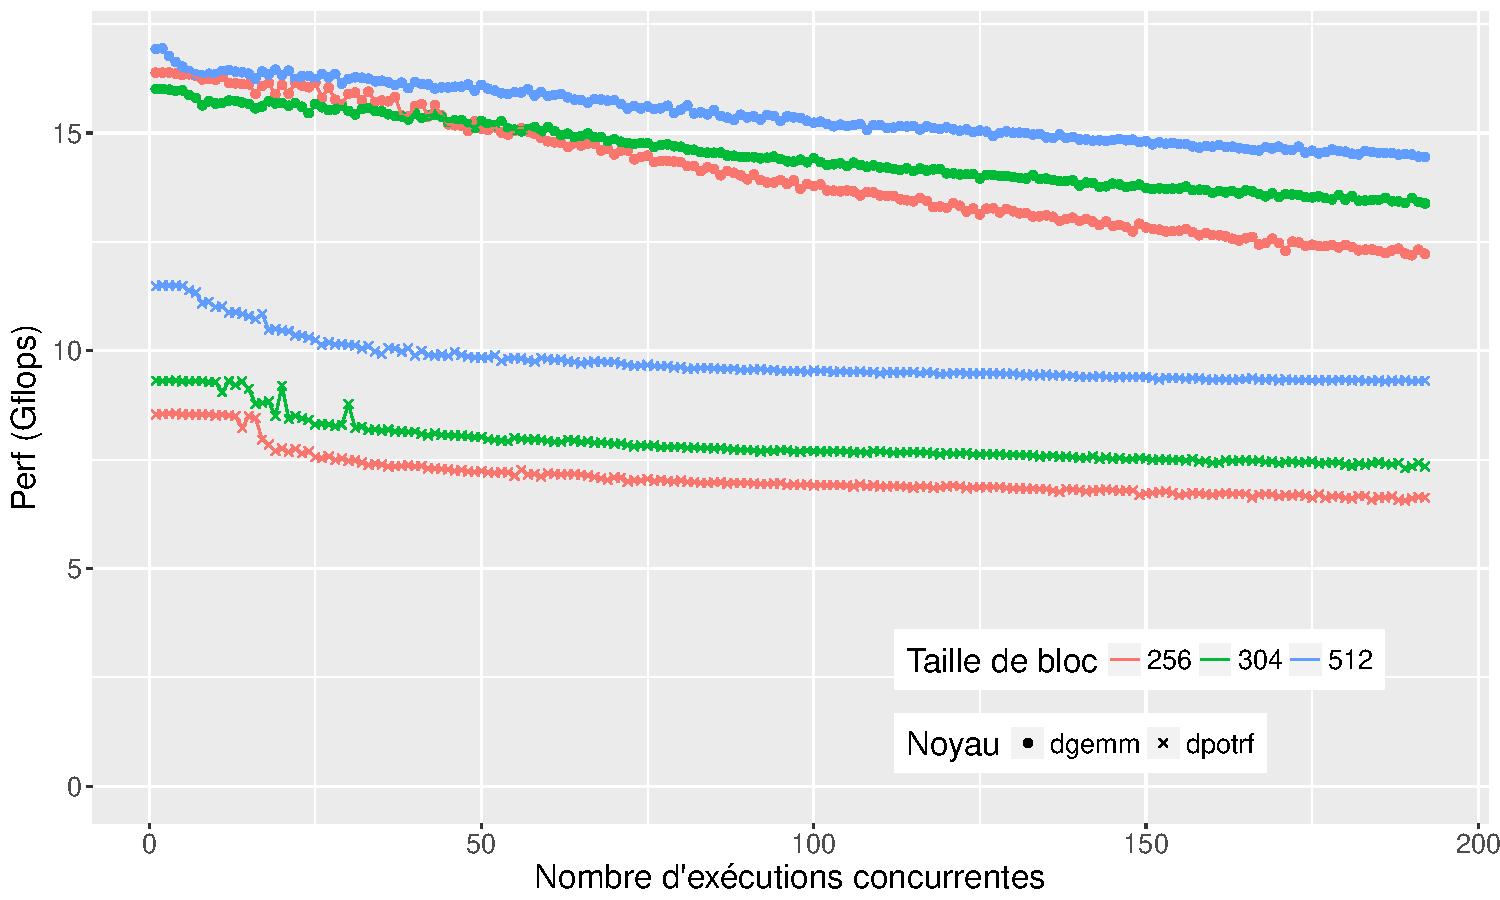
\includegraphics[width=0.95\textwidth]{kernels_multiple_bs_local_idchire}
  \caption{Performances des noyaux avec données locales sur idchire}\label{fig:contribs:apps:cholesky:perf-multiple-bs-idchire}
\end{figure}

La taille de bloc n'a pas d'impact significatif sur le phénomène observé précédemment de dégradation des performances.
Elle a bien un impact sur le niveau de performance globale de chaque noyau, mais le comportement général de chaque noyau reste le même.


\begin{todo}
  Même pas sûr de pourquoi il y a un niveau de perf différent... Je suppose que ça dépend des blas.
\end{todo}



\subsubsection{Impact de la bibliothèque BLAS}

\begin{todo}
GRAPHE : 4.3.5, dgemm/dsyrk/dtrsm faire : étude de comportement sur des paramètres représentatifs (obj : montrer l'impact des blas)
OpenBLAS, MKL, ATLAS
matter for top perf, not for overall behavior
\end{todo}




\bigskip
\bigskip

\outil nous a permis de mettre en évidence certaines caractéristiques des machines et des parties critiques d'une application utilisée comme étude de cas.
Le chapitre suivant est axé sur les différentes extensions que nous avons proposées dans le modèle de programmation et le support exécutif, afin d'essayer de mitiger le manque de localité des données.
En pratique les observations faites à travers \outil nous ont également servies à sélectionner des expériences et paramètres pertinents lors de l'évaluation des stratégies de vol de travail proposées avec la factorisation de Cholesky.
